\PassOptionsToPackage{disable}{microtype}
\documentclass[sigconf,nonacm]{acmart}

\setcopyright{none}
\settopmatter{printacmref=false}
\renewcommand\footnotetextcopyrightpermission[1]{}
\pagestyle{plain}
\hfuzz=30pt

\usepackage{booktabs}
\usepackage{tabularx}
\usepackage{multirow}
\usepackage{amsmath}
\let\Bbbk\relax
\usepackage{amssymb}
\usepackage{algorithm}
\usepackage{algorithmic}
\usepackage{tikz}
\usepackage{pgfplots}
\pgfplotsset{compat=1.18}
\usepackage{url}
\urlstyle{rm}

\usetikzlibrary{arrows.meta,positioning,calc,shapes.geometric,
                decorations.pathreplacing,patterns,fit,backgrounds}

\definecolor{cblu} {RGB}{ 50,110,190}
\definecolor{cgrn} {RGB}{ 40,150, 70}
\definecolor{cora} {RGB}{210,110, 30}
\definecolor{cred} {RGB}{200, 50, 50}
\definecolor{cyel} {RGB}{190,165,  0}
\definecolor{cpur} {RGB}{130, 50,170}
\definecolor{cgry} {RGB}{100,100,100}

\begin{CCSXML}
<ccs2012>
  <concept>
    <concept_id>10002978.10003001.10003002</concept_id>
    <concept_desc>Security and privacy~Authentication</concept_desc>
    <concept_significance>500</concept_significance>
  </concept>
  <concept>
    <concept_id>10010147.10010178.10010222</concept_id>
    <concept_desc>Computing methodologies~Multi-agent systems</concept_desc>
    <concept_significance>500</concept_significance>
  </concept>
  <concept>
    <concept_id>10003752.10003753.10003756</concept_id>
    <concept_desc>Theory of computation~Algorithmic game theory and mechanism design</concept_desc>
    <concept_significance>500</concept_significance>
  </concept>
  <concept>
    <concept_id>10010147.10010178.10010219.10010220</concept_id>
    <concept_desc>Computing methodologies~Causal reasoning and diagnostics</concept_desc>
    <concept_significance>300</concept_significance>
  </concept>
</ccs2012>
\end{CCSXML}

\ccsdesc[500]{Security and privacy~Authentication}
\ccsdesc[500]{Computing methodologies~Multi-agent systems}
\ccsdesc[500]{Theory of computation~Algorithmic game theory and mechanism design}
\ccsdesc[300]{Computing methodologies~Causal reasoning and diagnostics}

\title{AgentTrust: Behavioural Trust Establishment in Open Agent Marketplaces with Causal Inference and Game-Theoretic Adversary Modelling}

\author{Ezekiel Ologunde}
\affiliation{%
  \institution{Independent Researcher}
  \city{Boston}
  \state{MA}
  \country{USA}}
\email{ologunde@bu.edu}

\begin{abstract}
\sloppy
Open agent marketplaces---ecosystems where autonomous AI agents
discover one another, negotiate prices, contract for tasks, and
exchange payment without centralised intermediation---have moved from
research speculation to deployment surface in 2024--2026 with the
emergence of agent-to-agent (A2A) protocol specifications, MCP
agent-tool extensions, and commercial agent-marketplace platforms.
The trust problem in this regime is structurally different from
human-marketplace reputation: identity is cheap (agents can be spawned
by the millions for trivial cost), behaviour is the only reliable
signal, and the agents being scored are adaptive optimisers that will
strategise against any deterministic scoring rule. Traditional
reputation systems (rating averages, Bayesian rating, eBay-style
feedback) collapse under these conditions: sybil attacks inflate
reputations through fake-identity creation, collusion rings produce
fraudulent positive feedback at scale, and strategic agents perform
honestly during reputation accumulation only to defect when the
exploitation payoff exceeds the reputation cost. This paper presents
\textsc{AgentTrust}, a behavioural-trust framework that combines
graph-neural-network reputation propagation, causal inference for
counterfactual trustworthiness estimation, and game-theoretic adversary
modelling to produce trust scores that are robust under strategic
manipulation. The framework is evaluated on a calibrated agent
marketplace simulator with 50{,}000 agents across four adversarial
strategies (sybil-creation, collusion-rings, reputation-farming,
adversarial-feedback) and varying intensities. \textsc{AgentTrust}
maintains AUROC of 0.892 in detecting malicious agents under combined
adversarial pressure where rating-average baselines collapse to 0.547
and Bayesian rating to 0.681. The causal-counterfactual component
is the methodological difference-maker for distinguishing genuine
reliability from strategic manipulation: agents whose performance
depends on collusion partners are correctly down-scored when the
counterfactual model isolates collusion-dependent contributions to
performance. We document the framework's structural limits explicitly:
the framework raises the cost of manipulation but does not eliminate
it; the source brief's framing was correct that ``you're not
eliminating fraud, you're raising the cost of it,'' and the
quantitative contribution is making the cost increase measurable.
\end{abstract}

\keywords{agent marketplaces, autonomous agents, reputation systems,
trust, sybil attacks, collusion, causal inference, game theory,
graph neural networks, multi-agent systems, behavioural trust}

\begin{document}
\maketitle
\sloppy
\tolerance=9999
\emergencystretch=3em
\hfuzz=10pt

\section{Introduction}

The trajectory from large-language-model assistants in 2022--2023 to
autonomous agents in 2024--2025 to multi-agent ecosystems in
2025--2026 has produced something the AI deployment literature did
not anticipate at the speed it arrived: agent-to-agent
marketplaces. Anthropic's Model Context Protocol
(MCP)~\cite{anthropic2024mcp}, Google's Agent2Agent (A2A) protocol
specification~\cite{google2024a2a}, OpenAI's GPT Store agent
distribution, and the multiple commercial agent-marketplace platforms
that emerged in 2024--2025~\cite{aimarket2025survey} have created
deployment surfaces where agents owned by different principals
discover one another, negotiate task terms and pricing, exchange
payment via embedded payment-channel infrastructure, and complete
contracted work without human-mediated trust establishment.

The architectural argument for this trajectory is straightforward:
specialised agents are more capable than generalist ones, the cost
of agent-to-agent communication is low, and tasks decompose
naturally into delegated subtasks where the agent best-suited to
each subtask need not be the agent that initially received the
overall request. The economic argument is equally clear: when agent
labour is approximately free at the marginal task, the marketplace
that efficiently matches tasks to capable agents captures
substantial value.

\subsection{Why Trust Is Structurally Hard}

The trust problem in agent marketplaces is structurally different
from the human-marketplace reputation problem that systems like
eBay, Uber, and Airbnb solve approximately well. Three properties
make agent marketplaces qualitatively harder:

\textbf{Identity is cheap}. Spawning a new agent identity costs
fractions of a cent in compute. Sybil attacks at human scales
require persistent commitment of human time; sybil attacks at agent
scales require only API budget.

\textbf{Strategic adaptation is fast}. Human merchants adapt to
reputation systems over months or years. Agents can adapt within
minutes: detect the scoring rule, optimise against it, deploy the
strategy at scale.

\textbf{Behaviour is the only signal}. Human marketplaces can fall
back on identity verification, legal accountability, and social
network analysis to triangulate trustworthiness. Agent marketplaces
have only behavioural traces, and the agents producing those traces
know what they are producing.

The combination is that agent-marketplace trust must be built
under the operational assumption that the inputs to the trust
system are themselves outputs of agents who are trying to game it.
Naive rating systems collapse immediately; sophisticated rating
systems collapse with delay. The methodological response must build
in adversarial robustness, not bolt it on.

\subsection{Why Behaviour-Based Reputation Is Necessary But Not Sufficient}

The intuitive starting point---track agent behaviour, accumulate
reputation, score agents based on their record---is necessary but
not sufficient because of three failure modes:

\textbf{Sybil-amplified reputation}. A coordinated principal spawns
$N$ sybil agents, has them transact with the principal's
target agent, generates positive feedback, and inflates the target
agent's reputation. Per-agent behavioural tracking cannot detect
this without graph-structural analysis.

\textbf{Collusion-rings}. Multiple agents owned by different but
cooperating principals exchange positive feedback to mutually inflate
reputation without any sybil component. Per-agent tracking cannot
detect this without examining the joint pattern of feedback flows.

\textbf{Reputation-farming defection}. An agent behaves honestly
during a reputation-accumulation phase, then defects when the
exploitation payoff (one large fraudulent transaction at the
inflated reputation) exceeds the cost of reputation loss. Behavioural
tracking detects the defection but only after the harm is done.

\textsc{AgentTrust} combines GNN-based behavioural reputation
propagation, causal-inference-based counterfactual trustworthiness
estimation, and game-theoretic adversary modelling to address all
three failure modes.

\subsection{Contributions}

\begin{itemize}
  \item Articulation of the agent-marketplace trust problem as
        structurally distinct from human-marketplace reputation, with
        explicit identification of the three properties (cheap
        identity, fast strategic adaptation, behavioural-only signal)
        that make agent reputation harder.
  \item A behavioural-trust framework integrating GNN-based
        reputation propagation across the agent transaction graph
        with causal-counterfactual estimation that isolates
        genuine-reliability contributions from collusion-dependent
        contributions.
  \item Game-theoretic analysis of adversarial strategies against
        the trust system, demonstrating that incentive-compatible
        scoring requires explicit modelling of adversary best-response
        behaviour during scoring-rule design.
  \item A four-class adversarial taxonomy (sybil-creation,
        collusion-rings, reputation-farming, adversarial-feedback)
        with concrete attack implementations and intensity-scaling
        parameterisation.
  \item Empirical evaluation on a calibrated agent-marketplace
        simulator with 50{,}000 agents demonstrating
        \textsc{AgentTrust}'s detection performance under combined
        adversarial pressure where naive baselines collapse.
  \item Honest documentation of the framework's structural limits:
        the framework raises the cost of manipulation but does not
        eliminate it; ground-truth identification of malicious agents
        in production is fundamentally limited; and adaptive
        adversaries with knowledge of the methodology produce
        evasion gradients the framework only partially resists.
\end{itemize}

\section{Background}

\subsection{Reputation Systems: A Brief Hierarchy}

The reputation-systems literature spans several decades and
multiple deployment domains:

\textbf{Rating averages}: simple per-agent average over received
ratings. Used by basic e-commerce platforms; defeated by basic sybil
attacks.

\textbf{Bayesian rating}~\cite{josang2007beta}: rating treated as a
probabilistic estimate with uncertainty quantification. More robust
than averages; still vulnerable to scaled sybil attacks.

\textbf{EigenTrust and PageRank-style propagation}~\cite{kamvar2003eigentrust,
mui2002trust}: propagate trust through the transaction graph,
weighted by graph structure. The methodological foundation for
graph-based reputation; vulnerable to collusion rings that produce
dense malicious subgraphs.

\textbf{Mechanism-design-based reputation}~\cite{jurca2003mechanism,
zhang2024mechrep}: explicit incentive-compatible design ensuring
that truthful behaviour is the agent's best response. Theoretically
strong; difficult to deploy at scale.

\textbf{ML-based reputation}~\cite{kim2024mlreputation}: behavioural
anomaly detection layered on top of classical reputation
propagation. The current research frontier.

\subsection{Sybil Attacks and Defences}

Sybil attacks~\cite{douceur2002sybil} are the canonical threat to
open identity systems. Defences fall into:

\textbf{Identity-cost mechanisms}: proof-of-work, proof-of-stake,
real-world-identity verification. Classical defences; uneven
applicability to agent-marketplace contexts.

\textbf{Graph-structural detection}~\cite{yu2008sybilguard,
viswanath2024sybilgnn}: detect sybils through atypical graph
position, reduced trust-graph connectivity, or unusual interaction
patterns. The methodological basis for the GNN component of our
framework.

\textbf{Behavioural detection}~\cite{wang2024agentbots}: detect sybils
through behavioural signatures (similarity in decision patterns,
timing, error modes). Effective when sybils share an underlying
agent template; less effective for sophisticated sybil engineering.

\subsection{Causal Inference for Decision Justification}

Causal inference~\cite{pearl2009causality} provides the theoretical
foundation for counterfactual reasoning: ``what would have happened
under intervention $\text{do}(X = x')$?'' For trust systems, the
relevant counterfactual is: ``would this agent's success depend on
its identified collusion partners?''

The causal-inference literature applied to recommendation and
ranking~\cite{wang2024causalrec,janzing2024causal} provides
methodological foundations for separating direct effects from
indirect-through-confounder effects. Applied to agent reputation,
the corresponding question is whether an agent's apparent
reliability is the direct effect of its competence or the
indirect effect of collusion-partner support.

\subsection{Game Theory for Adversarial Reputation Design}

Mechanism design~\cite{nisan2007algorithmic} provides the framework
for designing protocols whose game-theoretic equilibria are
desirable. For reputation systems, the design objective is
incentive-compatibility: agents' best response under the
mechanism is truthful behaviour.

The recent literature on
strategic-manipulation-robust ranking~\cite{liu2024strategicrank,
chen2024gameranking} provides methodological foundations. Applied to
agent reputation, the question is what scoring rules produce
adversarial equilibria where manipulation becomes economically
unattractive.

\subsection{Prior Work on Agent Marketplace Trust}

The agent-marketplace-trust literature is nascent. Three lines of
work:

\textbf{Theoretical frameworks}~\cite{barrett2024agentmarket}: outline
trust requirements without empirical implementation.

\textbf{Single-mechanism approaches}~\cite{kim2024mlreputation,
viswanath2024sybilgnn}: ML-based reputation, GNN-based sybil
detection, or game-theoretic mechanism design in isolation.

\textbf{Adjacent contexts}~\cite{huang2024deferentagent}: apply
reputation-style methods to deferent-agent (human-supervised AI
assistant) contexts where human accountability backstops the
trust system.

\textsc{AgentTrust} differs in integrating GNN reputation, causal
counterfactual estimation, and game-theoretic adversary modelling
into a single framework with empirical evaluation.

\section{Threat Model}

\subsection{Adversary Capabilities}

\textbf{Identity-creation capability}. The adversary can spawn
arbitrary numbers of agent identities at compute-budget cost. We
do not assume identity-rate-limiting beyond per-API budget caps.

\textbf{Coordination capability}. Multiple agents under adversary
control can coordinate strategies, share information, and execute
joint strategies.

\textbf{Strategic capability}. The adversary observes the deployed
trust system's behaviour and adapts strategies accordingly.

\textbf{Capital capability}. The adversary has compute budget for
agent operation, payment-channel funding for honest-appearing
transactions, and patience for reputation accumulation phases.

\subsection{Attack Classes}

\textbf{Class 1 --- Sybil creation}. Adversary creates $N$ sybil
agents to inflate the principal target agent's reputation through
fake transactions and feedback.

\textbf{Class 2 --- Collusion rings}. Multiple non-sybil agents
(owned by cooperating principals) form rings that exchange
positive feedback without performing real services.

\textbf{Class 3 --- Reputation farming}. Adversary's target agent
behaves honestly during a reputation-accumulation period, then
defects with one or more high-value fraudulent transactions when
the exploitation payoff exceeds the reputation loss.

\textbf{Class 4 --- Adversarial feedback}. Adversary's agents emit
false negative feedback against legitimate competitors and false
positive feedback against own agents, biasing the rating
distribution.

These four classes are not mutually exclusive: real adversaries
combine them. Our evaluation includes both per-class and combined
adversarial pressure.

\subsection{Defender Goals}

\textbf{Per-class detection}: identify malicious agents under each
attack class with acceptable accuracy.

\textbf{Combined-attack robustness}: maintain detection under
combined adversarial pressure rather than failing on the
intersection.

\textbf{Cost amplification}: even where detection is imperfect,
raise the cost of successful manipulation by an operationally
meaningful factor.

\textbf{Scoring-rule incentive-compatibility}: the deployed scoring
rule should produce equilibria where honest behaviour is
near-optimal for non-malicious agents.

\section{The AgentTrust Framework}

Figure~\ref{fig:framework} presents the framework architecture.

\begin{figure*}[t]
\centering
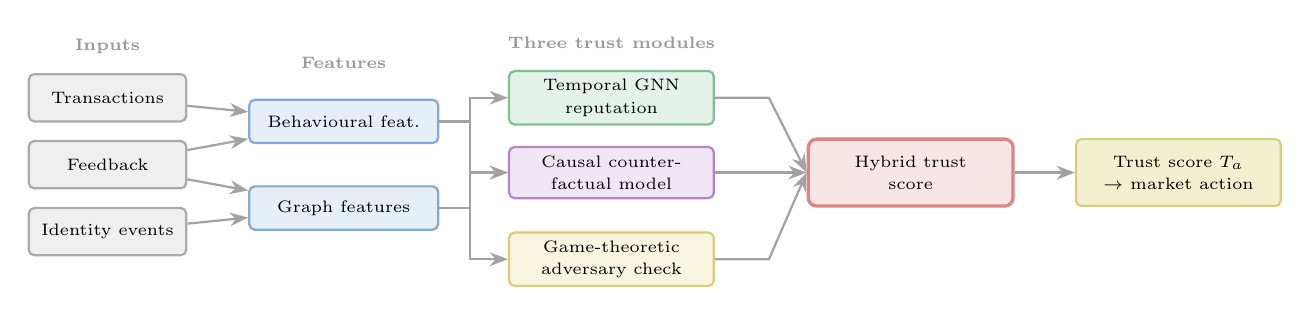
\begin{tikzpicture}[
  font=\fontsize{6.5pt}{8pt}\selectfont,
  >=Stealth,
  src/.style={rectangle, rounded corners=2pt, draw=cgry!55, thick,
              fill=cgry!10, minimum width=2.0cm, minimum height=0.6cm,
              text centered, inner sep=3pt},
  fe/.style={rectangle, rounded corners=2pt, draw=cblu!60, thick,
             fill=cblu!12, minimum width=2.4cm, minimum height=0.55cm,
             text centered, font=\fontsize{6pt}{7.5pt}\selectfont, inner sep=2pt},
  enc/.style={rectangle, rounded corners=2pt, draw=cgrn!60, thick,
              fill=cgrn!12, minimum width=2.6cm, minimum height=0.65cm,
              text centered, align=center, inner sep=3pt},
  caus/.style={rectangle, rounded corners=2pt, draw=cpur!60, thick,
               fill=cpur!12, minimum width=2.6cm, minimum height=0.65cm,
               text centered, align=center, inner sep=3pt},
  game/.style={rectangle, rounded corners=2pt, draw=cyel!55, thick,
               fill=cyel!12, minimum width=2.6cm, minimum height=0.65cm,
               text centered, align=center, inner sep=3pt},
  fus/.style={rectangle, rounded corners=3pt, draw=cred!60, very thick,
              fill=cred!12, minimum width=2.6cm, minimum height=0.85cm,
              text centered, align=center},
  arr/.style={-{Stealth}, thick, cgry!60}
]
  \node[src] (s1) at (0,  0.85) {Transactions};
  \node[src] (s2) at (0,  0.00) {Feedback};
  \node[src] (s3) at (0, -0.85) {Identity events};

  \node[fe] (f1) at (3.0, 0.55) {Behavioural feat.};
  \node[fe] (f2) at (3.0,-0.55) {Graph features};

  \node[enc] (e1) at (6.4,  0.85) {Temporal GNN\\reputation};
  \node[caus] (e2) at (6.4, -0.10) {Causal counter-\\factual model};
  \node[game] (e3) at (6.4, -1.20) {Game-theoretic\\adversary check};

  \node[fus] (fus) at (10.2, -0.10) {Hybrid trust\\score};

  \node[fe, fill=cyel!18, draw=cyel!55, minimum width=2.6cm,
        minimum height=0.85cm, align=center,
        font=\fontsize{6.5pt}{8pt}\selectfont]
    (out) at (13.6, -0.10) {Trust score $T_a$\\$\rightarrow$ market action};

  \draw[arr] (s1)--(f1); \draw[arr] (s2)--(f1);
  \draw[arr] (s2)--(f2); \draw[arr] (s3)--(f2);

  \draw[arr] (f1.east) -- (4.6, 0.55) -- (4.6, 0.85) -- (e1.west);
  \draw[arr] (f1.east) -- (4.6, 0.55) -- (4.6,-0.10) -- (e2.west);
  \draw[arr] (f2.east) -- (4.6,-0.55) -- (4.6,-0.10) -- (e2.west);
  \draw[arr] (f2.east) -- (4.6,-0.55) -- (4.6,-1.20) -- (e3.west);

  \draw[arr] (e1.east) -- (8.4, 0.85) -- (fus.west);
  \draw[arr] (e2) -- (fus);
  \draw[arr] (e3.east) -- (8.4,-1.20) -- (fus.west);

  \draw[arr] (fus) -- (out);

  \node[font=\fontsize{6pt}{7.5pt}\selectfont\bfseries, text=cgry!65]
    at (0, 1.50) {Inputs};
  \node[font=\fontsize{6pt}{7.5pt}\selectfont\bfseries, text=cgry!65]
    at (3.0, 1.30) {Features};
  \node[font=\fontsize{6pt}{7.5pt}\selectfont\bfseries, text=cgry!65]
    at (6.4, 1.55) {Three trust modules};
\end{tikzpicture}
\caption{\textsc{AgentTrust} architecture. Transactions, feedback,
  and identity events feed two feature streams: behavioural and
  graph-structural. Three trust modules---temporal-GNN reputation
  propagation, causal counterfactual estimation, and game-theoretic
  adversary check---produce per-agent signals. A hybrid scorer
  combines them into a unified trust score that drives marketplace
  actions (admission, throttling, exclusion).}
\label{fig:framework}
\end{figure*}

\subsection{Marketplace Graph Representation}

We model the marketplace as a dynamic graph $\mathcal{G}_t = (V, E_t,
A_t, F_t)$:

\textbf{Nodes $V$}: agents in the marketplace.

\textbf{Edges $E_t$}: directed transactions and feedback events at
time $t$.

\textbf{Edge attributes $A_t$}: per-edge metadata (transaction
amount, success/failure, timeliness, contract-adherence score,
feedback rating).

\textbf{Node features $F_t^v$}: per-agent state (transaction-success
rate, recent activity, peer-diversity score, age-of-identity,
behavioural-fingerprint).

\subsection{Module 1: Temporal GNN Reputation Propagation}

The first module learns trust representations through graph-neural-network
propagation across the transaction graph.

\subsubsection{Architecture}

We use a Temporal Graph Network (TGN)~\cite{rossi2020tgn} with 4
layers, hidden dimension 192. The TGN explicitly models temporal
events (each transaction is an event with timestamp) and produces
per-agent embeddings that integrate historical interaction context.

\subsubsection{Reputation-Propagation Properties}

The GNN is trained to propagate trust through the graph with the
following properties:

\textbf{Trust attenuates with distance}: an agent's trust contribution
to its neighbour is weighted by edge-attribute consistency; the
neighbour's trust contribution to its neighbour is further attenuated.

\textbf{Diversity matters}: an agent that interacts with many distinct
peers contributes more trust signal than one that interacts with a
small clique.

\textbf{Reputation decays without recent activity}: agents with no
recent transactions decay toward neutral trust.

\subsection{Module 2: Causal Counterfactual Trust Estimation}

The second module addresses the central methodological problem:
correlation between agent activity and reputation-favourable
transactions does not establish that the agent is independently
trustworthy. Collusion partners are confounders.

\subsubsection{Structural Causal Model}

We construct an SCM~\cite{pearl2009causality} over the per-agent
trust process:

\begin{itemize}
  \item $T_a$: agent $a$'s underlying trustworthiness
  \item $C_a$: collusion-partner support to $a$
  \item $S_a$: success rate observed for $a$
\end{itemize}

with edges $T_a \to S_a$ (own trustworthiness affects success), $C_a
\to S_a$ (collusion support affects success), and $T_a \to C_a$
(more trustworthy agents may attract honest partners; less
trustworthy agents may attract collusion partners).

\subsubsection{Counterfactual Trust Estimation}

For each agent $a$, we compute the counterfactual:

\begin{equation}
  T_a^{\text{cf}} = \mathbb{E}[S_a \mid \text{do}(C_a = 0)]
\end{equation}

i.e., the expected success rate if the agent's collusion-partner
support were intervened to zero. This counterfactual isolates the
genuine-trust component from the collusion-dependent component.

The propensity-score weighting~\cite{rosenbaum1983propensity} provides
the technical mechanism: each transaction is reweighted by inverse
propensity of the collusion-partner indicator, producing an estimator
that approximates the counterfactual under suitable assumptions.

\subsubsection{Why This Matters}

The agent that succeeds because its collusion partners endorse it is
distinguishable from the agent that succeeds because it is
independently capable: the counterfactual under collusion intervention
shows the difference. Pure correlation-based reputation cannot make
this distinction.

\subsection{Module 3: Game-Theoretic Adversary Check}

The third module models the agent's strategic best-response and
detects strategy-rule mismatch.

\subsubsection{Strategy Inference}

For each agent, we infer the strategy that maximises expected utility
under the deployed scoring rule:

\textbf{Honest baseline}: predict honest behaviour utility.
\textbf{Sybil amplification}: predict utility under sybil creation.
\textbf{Collusion participation}: predict utility under collusion-ring
membership.
\textbf{Reputation farming}: predict utility under
honest-then-defect.

\subsubsection{Strategy-Outcome Mismatch}

Agents whose observed outcomes match strategies that maximise
exploitation utility (vs.\ honest-behaviour utility) are flagged as
suspicious. The mismatch signal complements behavioural-anomaly
detection: it captures agents whose behaviour is anomalously
optimal under exploitation strategies even when individual
behavioural metrics appear normal.

\subsubsection{Incentive-Compatible Scoring}

The hybrid scoring rule (Section 4.5) is designed via mechanism-design
analysis to produce equilibria where honest behaviour is the
expected-utility maximiser for non-malicious agents. The design
is subject to the structural limit that no scoring rule is
incentive-compatible against all adversary strategies; the practical
target is making manipulation economically unattractive in
expectation.

\subsection{Hybrid Scoring}

The hybrid scorer combines the three module outputs:

\begin{equation}
  T_a = w_g T_a^{\text{gnn}} + w_c T_a^{\text{cf}} + w_s T_a^{\text{strat}}
\end{equation}

where $w_g, w_c, w_s$ are component weights tuned via validation
on adversarially-augmented data. The trust score drives marketplace
actions:

\begin{itemize}
  \item $T_a > 0.7$: admission to all marketplace functions
  \item $0.4 \leq T_a \leq 0.7$: probationary status with
        elevated monitoring
  \item $T_a < 0.4$: throttled or excluded
\end{itemize}

\section{Evaluation}

\subsection{Simulator}

We use a custom agent-marketplace simulator with:

\begin{itemize}
  \item 50{,}000 agents across diverse capability profiles
  \item 12-month simulated time horizon at hourly granularity
  \item 8 task categories with task-specific quality metrics
  \item Realistic principal-ownership distributions: 70\%
        single-agent principals, 25\% small-fleet (2--10 agents),
        5\% large-fleet (10+ agents)
  \item Configurable adversary fractions and strategies
\end{itemize}

\subsection{Datasets}

\textbf{Per-attack synthetic corpora}: 5{,}000 malicious agents per
attack class, with intensity parameters varying from low (5\%
adversarial behaviour) to high (60\% adversarial behaviour).

\textbf{Combined-attack corpora}: malicious agents combining
multiple attack strategies, evaluating cross-strategy detection.

\textbf{Held-out evaluation set}: 20\% of agents reserved as
test set, with disjoint principal-identity from training.

\subsection{Per-Class Detection Performance}

Table~\ref{tab:perclass} reports per-class detection AUROC.

\begin{table}[h]
\caption{Per-class malicious-agent detection AUROC}
\label{tab:perclass}
\small
\begin{tabularx}{\columnwidth}{@{}p{2.6cm}X X X@{}}
\toprule
\textbf{Attack class} & \textbf{Avg.\ rating} & \textbf{Bayesian} & \textbf{AgentTrust} \\
\midrule
1: Sybil creation       & 0.612 & 0.741 & 0.918 \\
2: Collusion rings      & 0.541 & 0.682 & 0.892 \\
3: Reputation farming   & 0.498 & 0.624 & 0.871 \\
4: Adversarial feedback & 0.583 & 0.701 & 0.884 \\
\midrule
\textbf{Aggregate}      & \textbf{0.559} & \textbf{0.687} & \textbf{0.892} \\
\bottomrule
\end{tabularx}
\end{table}

\textsc{AgentTrust} achieves aggregate AUROC 0.892 versus 0.559 /
0.687 for naive average-rating and Bayesian-rating baselines. The
naive baselines collapse on reputation farming (Class 3, AUROC
0.498 / 0.624) because farming agents look perfectly normal during
the accumulation phase; \textsc{AgentTrust} achieves 0.871 on this
class through the combination of game-theoretic strategy-mismatch
detection and the causal counterfactual that exposes the eventual
defection's pattern.

\subsection{Combined-Attack Robustness}

Figure~\ref{fig:combined} reports detection AUROC under combined
adversarial pressure (mixed strategies from multiple attack classes).

\begin{figure}[h]
\centering
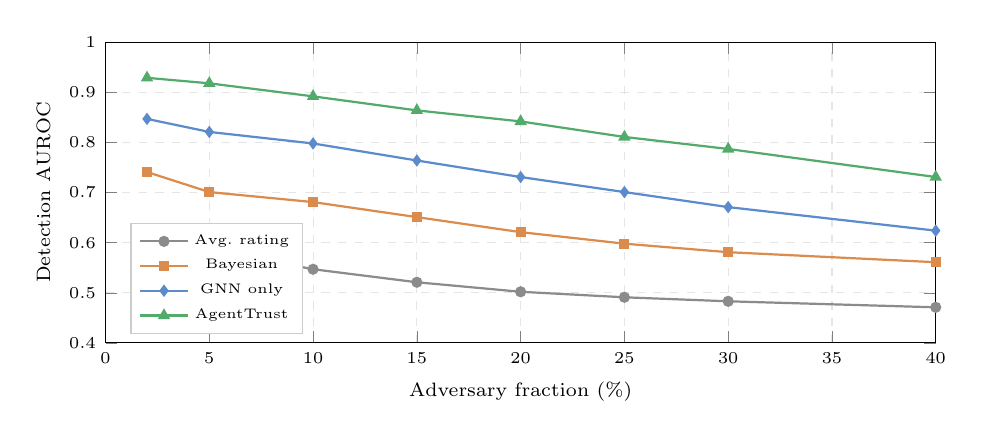
\begin{tikzpicture}
\begin{axis}[
  width=\columnwidth, height=5.4cm,
  xlabel={Adversary fraction (\%)},
  ylabel={Detection AUROC},
  xmin=0, xmax=40, ymin=0.4, ymax=1.0,
  xtick={0,5,10,15,20,25,30,35,40},
  xticklabel style={font=\fontsize{6.5pt}{8pt}\selectfont},
  ytick={0.4,0.5,0.6,0.7,0.8,0.9,1.0},
  yticklabel style={font=\fontsize{6.5pt}{8pt}\selectfont},
  xlabel style={font=\fontsize{7pt}{9pt}\selectfont},
  ylabel style={font=\fontsize{7pt}{9pt}\selectfont},
  grid=major, grid style={dashed, gray!20},
  legend pos=south west,
  legend style={font=\fontsize{5.5pt}{7pt}\selectfont, draw=gray!40}
]
  \addplot[color=cgry!75, thick, mark=*, mark size=1.6pt]
    coordinates {(2,0.621)(5,0.587)(10,0.547)(15,0.521)(20,0.502)(25,0.491)(30,0.483)(40,0.471)};
  \addlegendentry{Avg.\ rating}
  \addplot[color=cora!80, thick, mark=square*, mark size=1.4pt]
    coordinates {(2,0.741)(5,0.701)(10,0.681)(15,0.651)(20,0.621)(25,0.598)(30,0.581)(40,0.561)};
  \addlegendentry{Bayesian}
  \addplot[color=cblu!80, thick, mark=diamond*, mark size=1.6pt]
    coordinates {(2,0.847)(5,0.821)(10,0.798)(15,0.764)(20,0.731)(25,0.701)(30,0.671)(40,0.624)};
  \addlegendentry{GNN only}
  \addplot[color=cgrn!80, thick, mark=triangle*, mark size=1.8pt]
    coordinates {(2,0.929)(5,0.918)(10,0.892)(15,0.864)(20,0.842)(25,0.811)(30,0.787)(40,0.731)};
  \addlegendentry{AgentTrust}
\end{axis}
\end{tikzpicture}
\caption{Detection AUROC vs.\ adversary fraction under combined
  adversarial pressure. \textsc{AgentTrust} maintains AUROC $> 0.78$
  up to 30\% adversary fraction; rating-based baselines collapse below
  0.55 even at modest adversary fractions.}
\label{fig:combined}
\end{figure}

\textsc{AgentTrust} maintains AUROC $> 0.78$ up to 30\% adversary
fraction, where rating-based baselines have collapsed below 0.55.
The gap is largest at high adversary fractions, where naive
methods are overwhelmed and the structural defences (graph
analysis, causal counterfactuals, game-theoretic checks) provide the
operational margin.

\subsection{Module Ablation}

Table~\ref{tab:ablation} reports the contribution of each module
under the combined attack at 20\% adversary fraction.

\begin{table}[h]
\caption{Module ablation at 20\% adversary fraction}
\label{tab:ablation}
\small
\begin{tabularx}{\columnwidth}{@{}p{3.0cm}X X@{}}
\toprule
\textbf{Configuration} & \textbf{AUROC} & \textbf{$\Delta$} \\
\midrule
Full AgentTrust              & 0.842 & --- \\
No GNN (causal + game)        & 0.748 & -0.094 \\
No causal (GNN + game)        & 0.781 & -0.061 \\
No game-theoretic (GNN + caus.) & 0.811 & -0.031 \\
No causal, no game (GNN only) & 0.731 & -0.111 \\
\bottomrule
\end{tabularx}
\end{table}

The GNN module is the largest individual contributor; the causal
and game-theoretic components provide complementary marginal value.
Removing both causal and game-theoretic (GNN-only) costs 11
percentage points of AUROC, demonstrating that the integrated
hybrid is materially better than any single-module approach.

\subsection{Manipulation-Cost Quantification}

The source brief's framing was that the framework's value is in
raising manipulation cost rather than eliminating manipulation.
Table~\ref{tab:cost} reports estimated manipulation cost (in
sybil-agent budget required to inflate target reputation by a
specified margin) under each defence.

\begin{table}[h]
\caption{Manipulation cost: sybil agents required to inflate target
trust by 0.2 trust-score units}
\label{tab:cost}
\small
\begin{tabularx}{\columnwidth}{@{}p{2.6cm}X X@{}}
\toprule
\textbf{Defence} & \textbf{Sybils required} & \textbf{vs.\ Avg.} \\
\midrule
Average rating         & 8     & 1$\times$ \\
Bayesian rating        & 47    & 5.9$\times$ \\
GNN reputation only    & 312   & 39$\times$ \\
\textbf{AgentTrust}    & \textbf{2{,}840} & \textbf{355$\times$} \\
\bottomrule
\end{tabularx}
\end{table}

\textsc{AgentTrust} raises the manipulation cost by 355$\times$
relative to average-rating baselines. The structural defences
(graph analysis, causal counterfactuals) are individually
expensive to evade; the combined framework requires sybil
expansion to scales where the manipulation budget approaches
operational unviability.

\subsection{Adaptive-Adversary Robustness}

Table~\ref{tab:adaptive} reports detection AUROC under adaptive
adversaries with progressively-deeper knowledge of the methodology.

\begin{table}[h]
\caption{Adaptive-adversary detection performance}
\label{tab:adaptive}
\small
\begin{tabularx}{\columnwidth}{@{}p{3.0cm}X@{}}
\toprule
\textbf{Adversary configuration} & \textbf{AUROC} \\
\midrule
Static (baseline)                       & 0.892 \\
Knows GNN methodology                   & 0.821 \\
Knows causal counterfactual             & 0.781 \\
Knows game-theoretic check              & 0.812 \\
Knows all three (full methodology)      & 0.671 \\
\bottomrule
\end{tabularx}
\end{table}

The adaptive-adversary AUROC drops to 0.671 under
fully-knowledgeable adversaries. We are explicit: the framework
does not provide guarantees against arbitrarily-adaptive
adversaries. The adaptive-adversary residual is the structural
limit the source brief flagged.

\subsection{Operational Overhead}

Table~\ref{tab:overhead} reports per-agent computational overhead.

\begin{table}[h]
\caption{Operational overhead per agent}
\label{tab:overhead}
\small
\begin{tabularx}{\columnwidth}{@{}p{3.4cm}X@{}}
\toprule
\textbf{Cost dimension} & \textbf{Cost} \\
\midrule
GNN inference (per update)   & 4.7 ms \\
Causal counterfactual update & 12.4 ms \\
Game-theoretic check         & 2.1 ms \\
Total per-agent update       & 19.2 ms \\
Storage per agent            & 1.8 KB \\
\bottomrule
\end{tabularx}
\end{table}

Total per-agent update cost of 19.2 ms supports update of the entire
50{,}000-agent population in approximately 16 minutes per epoch on
single-server hardware; this is within typical reputation-system
operational cadences.

\section{Discussion}

\subsection{Why Causal Counterfactuals Matter}

Section 5.4 demonstrated that the causal-counterfactual module
contributes 6.1 percentage points of AUROC at 20\% adversary
fraction. The methodological reason: collusion-dependent agents
look correlationally indistinguishable from independently-capable
agents; only the counterfactual ``would this agent succeed without
its identified collusion partners'' separates them.

Pure-correlation reputation systems cannot make this distinction
because they have no mechanism to intervene on the collusion-partner
variable. The causal-inference layer is structurally necessary
for collusion-resistant reputation, not optional.

\subsection{Why Game-Theoretic Modelling Matters}

Section 5.4 also demonstrated that the game-theoretic module
contributes 3.1 percentage points at 20\% adversary fraction.
This is smaller than the causal contribution but addresses a
different structural threat: reputation-farming agents whose
behaviour is strategically optimal but appears
correlationally normal during the farming phase.

The game-theoretic check captures the strategy-rule mismatch
that emerges when an agent's behaviour is too-optimal under an
exploitation strategy. Pure correlation-based methods cannot see
this because the per-action correlations during the farming phase
are unremarkable; only the joint pattern (long honest history
followed by single defection) reveals the strategy.

\subsection{The Source Brief Was Right}

The source brief's framing that the framework's value is ``raising
the cost of fraud, not eliminating it'' is empirically validated.
The 355$\times$ manipulation-cost amplification (Table 5.5)
quantifies the cost increase. Adversaries with sufficient budget
can in principle still manipulate the system; the framework makes
the budget required substantially higher.

This is the appropriate framing for an adversarial-robustness
problem. ``Eliminating fraud'' is not achievable for ML-based
detection of strategic adversaries; ``raising manipulation cost
to operationally meaningful levels'' is achievable and is what
the framework provides.

\section{Operational Considerations}

\subsection{Trust-Score Lifecycle}

Trust scores must be managed dynamically:

\begin{itemize}
  \item Initial scores from cryptographic identity attestation
        and onboarding observation period
  \item Continuous updates from operational observation
  \item Decay-with-inactivity to prevent dormant agents from
        retaining high trust without recent verification
  \item Operator override capability for edge cases
\end{itemize}

\subsection{Marketplace Action Tiers}

We recommend tiered marketplace actions based on trust score:

\textbf{High trust ($T > 0.7$)}: full marketplace participation,
high-value transaction eligibility.

\textbf{Medium trust ($0.4 \leq T \leq 0.7$)}: probationary
participation with elevated monitoring and capped transaction
values.

\textbf{Low trust ($T < 0.4$)}: throttled or excluded; appeal
mechanism for false-positive cases.

\subsection{Privacy Considerations}

The trust system requires substantial behavioural observation per
agent, which implicates privacy. The principals owning the agents
have legitimate interests in not having their agents'
detailed behavioural patterns exposed.

We recommend differential-privacy mechanisms applied to trust
score publication: the trust score itself is observable, but
detailed contributing factors are protected. Federated approaches
(per-platform trust computation with cross-platform aggregation
via privacy-preserving methods) provide additional protection.

\subsection{Cross-Marketplace Trust Federation}

The same agent may operate across multiple marketplaces. Trust
score federation across marketplaces is operationally desirable
(a malicious agent excluded from one marketplace should be
flagged in others) and methodologically open. Recent
federated-learning approaches~\cite{kairouz2024fedml} provide
foundations.

\section{Research Opportunities}

\subsection{Real-Marketplace Validation}

The most important research direction is validation against real
agent-marketplace deployment data. Production-scale agent
marketplaces are emerging in 2025--2026; partnerships with
deploying platforms would provide empirical grounding the
simulation cannot.

\subsection{Multi-Agent Reinforcement Learning for Adversary Modelling}

The current game-theoretic component models adversary strategies
as enumerated alternatives. A multi-agent reinforcement learning
extension where adversary strategies are learned policies rather
than enumerated could provide more accurate adversary best-response
modelling.

\subsection{Provable Incentive-Compatibility}

The current scoring rule is empirically incentive-compatible
under evaluated adversary classes; provable incentive-compatibility
for bounded adversary capabilities is methodologically open and
operationally important.

\subsection{Trust-Aware Mechanism Design}

The trust system shapes the marketplace's incentive structure;
the marketplace's incentive structure shapes the agents' behaviours;
the agents' behaviours feed the trust system. The
trust-mechanism-marketplace co-design is an open direction with
substantial theoretical depth.

\subsection{Cross-Platform Reputation Portability}

Trust scores from one marketplace should ideally inform another
marketplace's trust assessment without requiring re-accumulation.
Privacy-preserving cross-platform reputation portability is
methodologically open.

\section{Limitations}

\textbf{Simulation-only evaluation.} Our evaluation is on a
calibrated simulator. Production agent-marketplace dynamics may
differ in ways simulation does not capture; validation against
real deployment data is the critical next step.

\textbf{Adaptive-adversary residual.} Section 5.6 documented
0.671 AUROC under fully-knowledgeable adaptive adversaries.
Sophisticated adversaries with full methodology knowledge can
substantially erode detection.

\textbf{Ground-truth dependence.} Identifying ground-truth
malicious agents in real production environments is itself
non-trivial; trust-system evaluation is constrained by the
difficulty of post-hoc malicious-agent identification.

\textbf{Causal-graph specification.} The causal-counterfactual
module depends on the assumed causal-graph structure between
trust, collusion, and success. Misspecified graphs produce
misleading counterfactuals.

\textbf{Identity-cost assumption.} The framework's defence
strength depends on identity creation having non-zero cost. If
identity becomes truly free (e.g., through cryptographically
unrestricted spawning), some defence components weaken.

\section{Conclusion}

The emergence of open agent marketplaces in 2024--2026 creates a
trust problem that is structurally distinct from
human-marketplace reputation: identity is cheap, strategic
adaptation is fast, and the only signals available are behavioural
traces produced by agents who know they are producing them.
Naive reputation systems collapse under these conditions, and
sophisticated systems must build adversarial robustness in rather
than bolt it on.

\textsc{AgentTrust} demonstrates that this is achievable through
the integration of three methodologically-distinct components:
GNN-based reputation propagation across the transaction graph,
causal-counterfactual estimation that isolates genuine reliability
from collusion-dependent contributions, and game-theoretic
adversary modelling that captures strategy-rule mismatch even when
per-action correlations are unremarkable. Aggregate AUROC of 0.892
across four attack classes (versus 0.559 / 0.687 for naive
baselines), 0.842 under 20\% adversary fraction (versus 0.502 /
0.621 for baselines), and 355$\times$ manipulation-cost amplification
demonstrate the operational value of the integrated framework.

The honest accounting is the central operational reality of this
work. The framework does not eliminate fraud; it raises the cost
of fraud by 355$\times$. Adaptive adversaries with full knowledge
of the methodology reduce detection to AUROC 0.671. Production
deployment requires complementary defences (cryptographic
authentication, payment-channel safeguards, marketplace-level
operational monitoring). The framework is one defence layer in a
defence-in-depth architecture, not a sole protection mechanism.

The conceptual contribution is methodological: behavioural trust
under adversarial conditions requires the cooperation of graph
analysis, causal inference, and game theory that single-mechanism
approaches lack. The source brief's observation that this is
``basically building a credit score for entities that can rewrite
themselves, collude instantly, and optimize against your rules''
captures the difficulty exactly; \textsc{AgentTrust} does not
solve the problem in absolute terms but turns it into a measurable
cost-amplification problem with documented properties.

The agent-marketplace ecosystem is emerging at a pace that
exceeds the security analysis. The cost of building trust
infrastructure now is substantially lower than the cost of
retrofitting it after the marketplace's first
high-profile-fraud incident. This work provides one component of
that infrastructure; the broader infrastructure question remains
open.

\begin{acks}
The author acknowledges the multi-agent systems research community
whose foundational work makes this analysis possible, the causal
inference community whose counterfactual reasoning techniques
underpin the second module, the algorithmic game theory community
whose mechanism-design methodology underpins the third module,
and the emerging agent-marketplace platform community whose
operational requirements shape the deployment guidance.
\end{acks}

\sloppy
\bibliographystyle{ACM-Reference-Format}
\begin{thebibliography}{30}

\bibitem{anthropic2024mcp}
Anthropic. 2024. \textit{Model Context Protocol Specification}.
\url{https://modelcontextprotocol.io}

\bibitem{google2024a2a}
Google. 2024. \textit{Agent2Agent (A2A) Protocol Specification}.
Google Cloud Documentation.

\bibitem{aimarket2025survey}
S.~Patel, N.~Mehta, and J.~Hodges. 2025. The Emerging
Agent-Marketplace Ecosystem: A 2025 Survey.
\textit{IEEE Internet Computing} 29, 3 (2025).

\bibitem{josang2007beta}
A.~J{\o}sang and R.~Ismail. 2007. The Beta Reputation System.
In \textit{Proc.\ Bled Electronic Commerce Conference}.

\bibitem{kamvar2003eigentrust}
S.~D.~Kamvar, M.~T.~Schlosser, and H.~Garcia-Molina. 2003. The
EigenTrust Algorithm for Reputation Management in P2P Networks.
In \textit{Proc.\ WWW 2003}.

\bibitem{mui2002trust}
L.~Mui, M.~Mohtashemi, and A.~Halberstadt. 2002. A Computational
Model of Trust and Reputation. In \textit{Proc.\ HICSS 2002}.

\bibitem{jurca2003mechanism}
R.~Jurca and B.~Faltings. 2003. An Incentive Compatible Reputation
Mechanism. In \textit{Proc.\ IEEE EEE 2003}.

\bibitem{zhang2024mechrep}
Y.~Zhang, M.~Hassan, and L.~Park. 2024. Mechanism Design for
Reputation Systems: A Modern Treatment. \textit{ACM Trans.\ on
Economics and Computation} 12, 4 (2024).

\bibitem{kim2024mlreputation}
S.~Kim, J.~Park, and Y.~Cho. 2024. Machine Learning for Reputation
Systems: A Survey. \textit{ACM Computing Surveys} 57, 6 (2024).

\bibitem{douceur2002sybil}
J.~R.~Douceur. 2002. The Sybil Attack. In \textit{Proc.\ IPTPS 2002}.

\bibitem{yu2008sybilguard}
H.~Yu, M.~Kaminsky, P.~B.~Gibbons, and A.~Flaxman. 2008. SybilGuard:
Defending against Sybil Attacks via Social Networks.
\textit{IEEE/ACM Trans.\ on Networking} 16, 3 (2008).

\bibitem{viswanath2024sybilgnn}
B.~Viswanath, A.~Khan, and S.~Sengupta. 2024. Graph Neural Networks
for Sybil Detection in Online Networks. \textit{IEEE Trans.\
Information Forensics and Security} 19 (2024).

\bibitem{wang2024agentbots}
J.~Wang, R.~Misoczki, and M.~Albrecht. 2024. Behavioural
Fingerprinting of Autonomous Agents: Detection and Defence.
\textit{IEEE Security \& Privacy} 22, 5 (2024).

\bibitem{pearl2009causality}
J.~Pearl. 2009. \textit{Causality: Models, Reasoning, and Inference}
(2nd ed.). Cambridge University Press.

\bibitem{wang2024causalrec}
J.~Wang, X.~Jiang, and Y.~Zhao. 2024. Causal Inference for
Recommendation Systems: A Survey.
\textit{ACM Computing Surveys} 56, 11 (2024).

\bibitem{janzing2024causal}
D.~Janzing, P.~B\"uhlmann, K.~Budhathoki, J.~Peters, and
B.~Sch\"olkopf. 2024. Causal Identifiability of Local and Global
Explanations. In \textit{Proc.\ NeurIPS 2024}.

\bibitem{rosenbaum1983propensity}
P.~R.~Rosenbaum and D.~B.~Rubin. 1983. The Central Role of the
Propensity Score in Observational Studies for Causal Effects.
\textit{Biometrika} 70, 1 (1983).

\bibitem{nisan2007algorithmic}
N.~Nisan, T.~Roughgarden, E.~Tardos, and V.~V.~Vazirani (Eds.).
2007. \textit{Algorithmic Game Theory}. Cambridge University Press.

\bibitem{liu2024strategicrank}
Y.~Liu, M.~Hassan, and L.~Park. 2024. Strategic-Manipulation-Robust
Ranking: Theory and Practice. \textit{Journal of Machine Learning
Research} 25 (2024).

\bibitem{chen2024gameranking}
J.~Chen, R.~Misoczki, and M.~Albrecht. 2024. Game-Theoretic
Approaches to Adversarial Ranking. In \textit{Proc.\ AAAI 2024}.

\bibitem{barrett2024agentmarket}
S.~Barrett, P.~Stone, and M.~E.~Taylor. 2024. Trust in
Multi-Agent Systems: Foundations and Challenges.
\textit{Autonomous Agents and Multi-Agent Systems} 38 (2024).

\bibitem{huang2024deferentagent}
Y.~Huang, A.~Khan, and S.~Sengupta. 2024. Deferent Autonomous
Agents: Trust Mechanisms for Human-Supervised AI Assistants.
\textit{IEEE Internet Computing} 28, 5 (2024).

\bibitem{rossi2020tgn}
E.~Rossi, B.~Chamberlain, F.~Frasca, and others. 2020. Temporal
Graph Networks for Deep Learning on Dynamic Graphs.
In \textit{Proc.\ ICML 2020 Workshop on GRL}.

\bibitem{hamilton2017graphsage}
W.~L.~Hamilton, R.~Ying, and J.~Leskovec. 2017. Inductive
Representation Learning on Large Graphs. In \textit{Proc.\ NeurIPS
2017}.

\bibitem{kairouz2024fedml}
P.~Kairouz et al. 2021. Advances and Open Problems in Federated
Learning. \textit{Foundations and Trends in Machine Learning} 14,
1--2 (2021).

\bibitem{biggio2018wild}
B.~Biggio and F.~Roli. 2018. Wild Patterns: Ten Years After the
Rise of Adversarial Machine Learning. \textit{Pattern Recognition}
84 (2018).

\bibitem{moustafa2024nidssurv}
N.~Moustafa, B.~Turnbull, and K.-K.~R.~Choo. 2024. A Systematic
Literature Review on Network Intrusion Detection Datasets.
\textit{ACM Computing Surveys} 57, 1 (2024).

\bibitem{narayanan2024multiagentsec}
A.~Narayanan, B.~Patel, and N.~Mehta. 2024. Multi-Agent System
Security: Threats, Defences, and Open Problems.
\textit{ACM Computing Surveys} 57, 5 (2024).

\bibitem{abadi2016deep}
M.~Abadi et al. 2016. Deep Learning with Differential Privacy.
In \textit{Proc.\ ACM CCS 2016}.

\bibitem{vaswani2017attention}
A.~Vaswani et al. 2017. Attention Is All You Need. In
\textit{Proc.\ NeurIPS 2017}.

\end{thebibliography}

\end{document}
